\subsection{Prioritize Requirements}\label{subsec:prioritize-requirements}

The other distinctive feature about HelixRM is the efficiency in simplifying and making fast the prioritization of requirements.
It provides for assessing and rating requirements in regard to factors related to business value, complexity, urgency, risk amongst others.
To make certain that stakeholders can make decisions which tally with organizational goals and project constraints weighted scoring, as well as customized parameters, is employed by HelixRM\@.
\paragraph{Establish Clear Evaluation Criteria}
HelixRM enables the users to define and customize evaluation criteria to suit the unique needs of their projects.

\paragraph{Weighted Scoring}
The platform allows for weighted scoring, which means the user can assign relative importance to each evaluation criterion.
This feature ensures that requirements are prioritized based on their significance to the project.

\paragraph{Automated Ranking}
HelixRM automates the ranking process, generating a prioritized list of requirements based on the established evaluation criteria and weighted scores.
This saves time and reduces subjectivity in the prioritization process.

\paragraph{Collaborative Decision-Making}
The tool provides a clear view into the prioritized requirements, leading to collaborative decision-making.
Stakeholders can discuss, review, and come to an agreement on what will be implemented in which order.

\paragraph{Scenario Analysis}
HelixRM supports scenario analysis, which lets users evaluate project outcomes under different prioritization strategies.
This allows stakeholders to make data-informed decisions that maximize the value of the project.

\paragraph{Continuous Refinement}
As project requirements evolve, HelixRM enables users to continuously refine and update the prioritization of requirements.
This iterative process ensures that project goals remain aligned with changing business needs.
The image Figure~\ref{fig:requirements_view} shows an example of a prioritization of a requirement.
\begin{figure}[htpb]
    \centering
    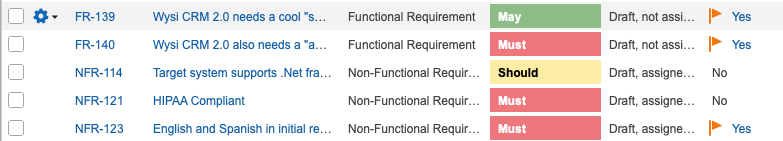
\includegraphics[width=\linewidth]{images/prioritize-example}
    \caption{Helix requirements view.}
    \label{fig:requirements_view}
\end{figure}